%versi 2 (8-10-2016)
\chapter{Landasan Teori}
\label{chap:teori}

\section{BlueTape}
\label{sec:blurtape}


\section{CodeIgniter}
\label{sec:code_igniter}
Codeigniter adalah sebuah kerangka kerja untuk pengembangan aplikasi - sebuah alat - bagi masyarakat yang ingin membangun website menggunakan PHP. Bertujuan agar proyek yang sedang dikembangkan lebih cepat daripada Anda menulis kode dari awal / \textit{scratch}, dengan menyediakan seperangkat libraries untuk tugas yang umumnya digunakan, semudah sebuah \textit{interface} dan struktur logika untuk mengakses \textit{libraries} tersebut. Codeigniter memungkinkan untuk fokus pada proyek Anda dengan mengurangi kode yang dibutuhkan untuk tugas tertentu. \cite{codeIgniter:17}
\subsection{Application Flow Chart}
\label{subs:app_flowchart}
Gambar berikut mengilustrasikan bagaimana alur data pada sistem :

\begin{figure} [H]
	\centering  
	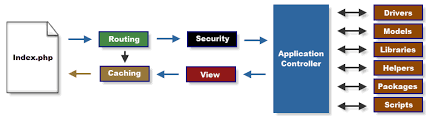
\includegraphics[scale=1.0]{appflowchart.png}  
	\caption[Flow Chart Codeignter. Sumber:\/\/www.codeigniter.com\/user\_guide\/\_images\/appflowchart.gif]{Flow Chart Codeignter. Sumber:\textit{ \/\/www.codeigniter.com\/user\_guide\/\_images\/appflowchart.gif}} 
	\label{fig:flow-chart-CodeIgniter} 
\end{figure}

\begin{enumerate}
\item index.php bertindak sebagai \textit{front controller}, menginisiasi \textit{base resources} yang dibutuhkan untuk menjalankan CodeIgniter.
\item Router akan memeriksa permintaan HTTP untuk menetapkan hal apa yang harus dilakukan dengan permintaan tersebut.
\item Apabila terdapat \textit{cache}, maka \textit{cache} tersebut akan dikirimkan langsung ke browser, dengan melewati sistem eksekusi normal.
\item Keamanan. Sebelum \textit{controller} aplikasi dimuat, \textit{HTTP request} dan \textit{user} mana pun yang mengirimkan data diseleksi dahulu untuk keamanan.
\item Controller memuat \textit{model, core libraries, helpers}, dan \textit{resources} yang dibutuhkan untuk proses \textit{request} yang spesifik.
\item \textit{View} yang telah selesai dirender kemudian dikirim ke \textit{web browser} untuk dilihat. Jika \textit{caching} diaktifkan, tampilan dicache terlebih dahulu sehingga pada permintaan selanjutnya dapat dilayani.

\subsection{CodeIgniter URLs}
\label{subs:urls}
Codeigniter menggunakan pendekatan \textbf{berbasis-segmen}:
\begin{lstlisting}[frame=single] 
example.com/news/article/my_article
\end{lstlisting}

\subsubsection{Url Segments}
\label{sssec:url_1}
Segmen didalam URl, 

\subsection{Model-View-Controller}
\label{subs:mvc}
Codeigniter bedasarkan pola pembangunan Model-View-Controller. MVC adalah pendekatan perangkat lunak yang memisahkan aplikasi logik dari presentasi. Dalam prakteknya, memungkinkan untuk \textit{web pages} Anda berisi \textit{scripting} yang sedikit karena presentasi terpisah dari skrip PHP.

\subsection{Model}
\label{subs:model}
\textit{Model} merepresentasikan struktur data Anda. Biasanya kelas \textit {model} akan berisi fungsi yang membantu untuk \textit{retrieve, insert}, dan \textit{update} informasi di database.

Dalam Codeigniter \textit{models} merupakan opsi yang tersedia untuk mereka yang ingin lebih menggunakan sebuah pendekatan tradisional MVC.

\subsubsection{Anatomi Model}
\label{sssec:model_1}

Kelas model akan disimpan di direktori \textbf{application/models/directory}. Kelas ini dapat bersarang didalam \textit{sub-directories} jika Anda menginginkan tipe organisasi seperti ini. 

Prototipe dasar dari sebuah model kelas :
\begin{lstlisting}[label=phpheg, frame=single]  
<?php
class Model_name extends CI_Model {

}
\end{lstlisting}

Nama file juga harus sama dengan nama kelas. Sehingga apabila kita ada kelas \verb|User_model| maka file Anda akan seperti ini.

\begin{lstlisting}[label=phpheg, frame=single]  
application/models/User_model.php
\end{lstlisting}

\subsubsection{Loading a Model}
\label{sssec:model_2}

Model Anda biasanya akan dimuat dan dipanggil didalam metode \textit{controller} Anda. Untuk memuat sebuah model anda akan menggunakan metode berikut:

\begin{lstlisting}[label=phpheg, frame=single] 
$this->load->model('model_name');
\end{lstlisting}

\subsubsection{Koneksi ke Database}
\label{sssec:model_3}
Apabila model sudah dimuat, model tersebut tidak terhubung secara langsung ke database. Dengan cara secara manual mengatur konektfitas database melalui parameter ketiga:

\begin{lstlisting}[label=phpheg, frame=single]
$config['hostname'] = 'localhost';
$config['username'] = 'myusername';
$config['password'] = 'mypassword';
$config['database'] = 'mydatabase';
$config['dbdriver'] = 'mysqli';
$config['dbprefix'] = '';
$config['pconnect'] = FALSE;
$config['db_debug'] = TRUE;

$this->load->model('model_name', '', $config);
\end{lstlisting}


\subsection{View}
\label{subs:view}
\textit{View} adalah informasi yang sedang dilihat oleh \textit{user}. Sebuah \textit{View} normalnya menjadi sebuah halaman web, namun dalam CodeIgniter, sebuah \textit{view} dapat menjadi sebuah \textit{page fragment} seperti \textit{header} atau \textit{footer}. Dapat juga menjadi halaman RSS, atau tipe apapun dari "page".

\textit{Views} tidak pernah dipanggil secara langsung, harus dimuat dalam sebuah \textit{controller}. Ingat bahwa dalam \textit{MVC framework}, \textit{controller} bertanggung jawab untuk mengambil \textit{view} tertentu. 

\subsubsection{Membuat sebuah View}
\label{sssec:view_1}
Dengan menggunakan \textit{text editor}, buat sebuah file yang memanggil \verb|blogview.php|, dan isi dengan kode berikut:
\begin{lstlisting}[frame=single, language=html]% 
<html>
<head>
        <title>My Blog</title>
</head>
<body>
        <h1>Welcome to my Blog!</h1>
</body>
</html>
\end{lstlisting}

Kemudian simpan file tersebut di application/views/ directory.

\subsubsection{Loading sebuah View}
\label{sssec:view_1}

View dapat dimuat dengan membuat file \textit{view} dengan syntax berikut:

\begin{lstlisting}[frame=single] 
$this->load->view('name');
\end{lstlisting}

Dimana \textit{name} adalah nama dari file \textit{view}.

Lalu, buka file \textit{controller} yang dibuat sebelumnya bernama Blog.php, dan pindahkan \textit{echo statement} dengan \textit{view loading method.}

\begin{lstlisting}[label=phpheg, frame=single] 
<?php
class Blog extends CI_Controller {

        public function index()
        {
                $this->load->view('blogview');
        }
}
\end{lstlisting}

\subsubsection{Memuat Beberapa View}
\label{sssec:view_2}
Codeigniter akan menangani beberapa panggilan dari dalam controller dengan syntax \verb|$this->load->view()|. Apabila ada lebih dari satu panggilan yang terjadi, maka \textit{views} akan dilampirkan secara bersamaan. Berikut ini kode yang digunakan apabila pengembang web ingin mempunyai sebuah \textit{header view}, sebuah \textit{menu view}, sebuah \textit{content view}, dan sebuah \textit{footer view}. 
\begin{lstlisting}[label=phpheg, frame=single] 
<?php

class Page extends CI_Controller {

        public function index()
        {
                $data['page_title'] = 'Your title';
                $this->load->view('header');
                $this->load->view('menu');
                $this->load->view('content', $data);
                $this->load->view('footer');
        }

}
\end{lstlisting}

\subsubsection{Menyimpan Views didalam \textit{Sub-directories}}
\label{sssec:view_3}
View files dapat disimpan didalam \textit{sub-directories} dengan menyertakan nama direktori yang memuat \textit{view}.
\begin{lstlisting}[label=phpheg, frame=single] 
$this->load->view('directory_name/file_name');
\end{lstlisting}

\subsubsection{Menambahkan data dinamis ke View}
\label{sssec:view_4}
Data yang dikirim dari controller menuju view dalam bentuk \textbf{array} atau objek akan dilampirkan dalam parameter kedua dalam metode loading view. 
Berikut ini pengguanaan dengan array:
\begin{lstlisting}[label=phpheg, frame=single] 
$data = array(
        'title' => 'My Title',
        'heading' => 'My Heading',
        'message' => 'My Message'
);

$this->load->view('blogview', $data);
\end{lstlisting}

Kemudian, penggunaan dengan objek:
\begin{lstlisting}[label=phpheg, frame=single] 
$data = new Someclass();
$this->load->view('blogview', $data);
\end{lstlisting}

Sehingga apabila dimasukan ke controller, kode yang ditambahkan adalah:
\begin{lstlisting}[label=phpheg, frame=single] 
<?php
class Blog extends CI_Controller {

        public function index()
        {
                $data['title'] = "My Real Title";
                $data['heading'] = "My Real Heading";

                $this->load->view('blogview', $data);
        }
}
\end{lstlisting}

Untuk mengaksesnya dalam file HTML maka dapat digunakan syntax php
\begin{lstlisting}[frame=single] 
<html>
<head>
        <title><?php echo $title;?></title>
</head>
<body>
        <h1><?php echo $heading;?></h1>
</body>
</html>
\end{lstlisting}

\subsection{Controller}
\label{subs:controller}
\textit{Controller} bertindak sebagai sebuah penengah antara Model, View dan \textit{resources} lain yang dibutuhkan untuk proses \textit{HTTP requests} dan menghasilkan sebuah halaman web.

Sebuah \textit{controller} secara sederhana merupakan sebuah file yang dinamakan sehingga dapat dikaitkan dengan URl.
Misalnya untuk URl ini:
\begin{lstlisting}[label=phpheg, frame=single] 
<?php
example.com/index.php/blog/
\end{lstlisting}

Dalam contoh diatas, \textit{Codeigniter} berusaha menemukan \textit{controller} bernama Blog.php dan memuatnya. Ketika sebuah nama \textit{controller} sesuai dengan \textit{first segment} dari sebuah URl, maka URl akan memuatnya.

Kode berikut merupakan contoh dari \textit{controller} sederhana.
\begin{lstlisting}[label=phpheg, frame=single] 
<?php
class Blog extends CI_Controller {

        public function index()
        {
                echo 'Hello World!';
        }
}
\end{lstlisting} 

\subsubsection{Method}
\label{sssec:controller_1}
Dalam sebuah kelas \textit{controller} akan terdapat beberapa method, untuk memanggil fungsi didalamnya maka dapat mengisi segmen kedua dari sebuah url.
\begin{lstlisting}[label=phpheg, frame=single] 
<?php
class Blog extends CI_Controller {

        public function index()
        {
                echo 'Hello World!';
        }

        public function comments()
        {
                echo 'Look at this!';
        }
}
\end{lstlisting}

Pemanggilan method index dapat secara otomatis dilakukan apabila segmen kedua kosong.Cara lain untuk menjalankan method comments() dapat dilakukan dengan:
\begin{lstlisting}[frame=single] 
example.com/index.php/blog/index/
\end{lstlisting}

Kemudian untuk memuat method comment dapat dituliskan sebagai berikut:
\begin{lstlisting}[frame=single] 
example.com/index.php/blog/comments/
\end{lstlisting}

\section{Zurb Foundation 6}
\label{sec:zurb_foundation6}

\subsection{Struktur File}
\label{subs:strukturfile_zurb}
\begin{figure} [H]
	\centering  
	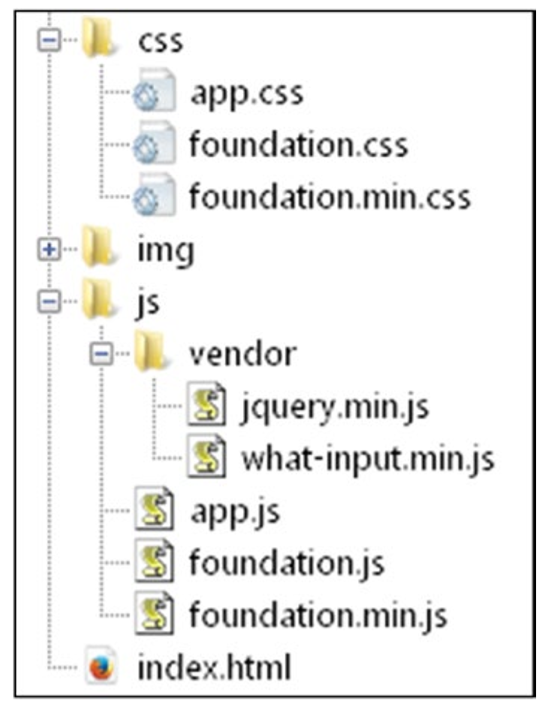
\includegraphics[scale=1.0]{filestructure_zurb.png}  
	\label{fig:filestructure_zurb} 
\end{figure}

Framework Foundation terdiri dari 3 folder utama:
Folder \textbf{css} terdiri dari semua \textit{CSS Style} yang digunakan dalam Foundation 6. Didalam folder terdapat versi yag diperkecil \verb|foundation.min.css| atau versi yang tidak dikompresi \verb|foundation.css|. Seluruh modifikasi \textit{stylesheets} ditempatkan pada folder ini agar lebih terstruktur.
Folder \textbf{img} tempat meletakkan semua gambar untuk projek web.
Folder \textbf{js} terdiri dari semua file Javascript yang sudah ditentukan sebelumnya.

\subsection{Sistem Grid pada Foundation}
\label{subs:grid_zurb}
\begin{lstlisting}[breaklines,breakatwhitespace, frame=single, basicstyle=\small] 
<!doctype html> <html class="no-js" lang="en">  
	<head>    
	<meta charset="utf-8" />    
	<meta name="viewport" content="width=device-width, initial-scale=1.0" />    
	<title>Foundation | Interchange</title> 
	<link rel="stylesheet" href="https://cdnjs.cloudflare.com/ajax/libs/ foundation/6.0.1/css/foundation.min.css">
	 
	<script src="https://cdnjs.cloudflare.com/ajax/libs/foundation/6.0.1/js/ vendor/jquery.min.js"></script> <script src="https://cdnjs.cloudflare.com/ajax/libs/foundation/6.0.1/js/ foundation.min.js"></script>
	 
	</head> 
 <body >  
	 <script src="https://cdnjs.cloudflare.com/ajax/libs/foundation/6.0.1/js/ vendor/what-input.min.js"></script> 
	 <script>      $(document).foundation();  </script>     
 </body> 
</html>
\end{lstlisting}

Pada bagian \verb|<head>|, terdapat tag meta charset yang digunakan untuk mendefinisikan set karakter dokumen HTML. Kemudian tag meta viewport membantu desainer untuk mengatur \texttt{viewport}, yaitu pembagian dari halaman web yang terlihat oleh pengguna. Sementara \texttt{width=device-width} menetapkan lebar halaman sesuai layar perangkat, \texttt{initial-scale=1.0} menunjukan bahwa device akan menampilkan layar tanpa diperbesar. Kemudian ada link yang menjelaskan mengenai CDN, berikut link nya:

\url{https://cdnjs.com/libraries/foundation}

Tag \texttt{<link>} akan mendefinisikan link CDN\texttt{foundation.min.css} yang berfungsi untuk file \texttt{CSS} secara default. Tautan \texttt{jquery.min.js} harus dimasukkan sebelum
tautan \texttt{foundation.min.js}, sebagaimana plug-in dan atribut JavaScript milik Foundation
bergantung pada jQuery.

Tepat sebelum kita memanggil fungsi Foundation, kita perlu memasukkan \texttt{what-input}.
tautan CDN \texttt{min.js}. File ini digunakan untuk melacak metode input saat ini, apakah itu 
mouse, keyboard, atau layar sentuh. ~\cite{zurb:15:introfoundation}

Buku:~\cite{berg:08:compgeom} 


\subsection{\textit{Navigation} dan \textit{Media Attributes}}
\label{subs:view}

\subsection{Komponen CSS}
\label{subs:css_zurb}

\subsection{Komponen JavaScript}
\label{subs:css_javascript}
 

\section{Bootstrap 4}
\label{sec:bootstrap4}
 
\section{Template Skripsi FTIS UNPAR}
\label{sec:template}
 
Akan dipaparkan bagaimana menggunakan template ini, termasuk petunjuk singkat membuat referensi, gambar dan tabel.
Juga hal-hal lain yang belum terpikir sampai saat ini. 
 
\dtext{15-16}

\subsection{Tabel}  
Berikut adalah contoh pembuatan tabel. 
Penempatan tabel dan gambar secara umum diatur secara otomatis oleh \LaTeX{}, perhatikan contoh di file bab2.tex untuk melihat bagaimana cara memaksa tabel ditempatkan sesuai keinginan kita.

Perhatikan bawa berbeda dengan penempatan judul gambar gambar, keterangan tabel harus diletakkan di atas tabel!!
Lihat Tabel~\ref{tab:contoh1} berikut ini:

\begin{table}[H] %atau h saja untuk "kira kira di sini"
	\centering 
	\caption{Tabel contoh}
	\label{tab:contoh1}
	\begin{tabular}{cccc}
		\toprule
		& $v_{start}$ & $\mathcal{S}_{1}$ & $v_{end}$\\

		\midrule
		$\tau_{1}$ & 1 & 12& 20\\
		$\tau_{2}$ & 1 &  & 20\\
		$\tau_{3}$ & 1 & 9 & 20\\
		$\tau_{4}$ & 1 &  & 20\\

		\bottomrule
		
	\end{tabular} 
\end{table}
Tabel~\ref{tab:cthwarna1} dan Tabel~\ref{tab:cthwarna2} berikut ini adalah tabel dengan sel yang berwarna dan ada dua tabel yang bersebelahan. 
\begin{table}[H]
	\begin{minipage}[c]{0.49\linewidth}
		\centering
		\caption{Tabel bewarna(1)}
		\label{tab:cthwarna1}
		\begin{tabular}{ccccc}
			\toprule
			 & $v_{start}$ & $\mathcal{S}_{2}$ & $\mathcal{S}_{1}$ & $v_{end}$\\
			
			\midrule
			$\tau_{1}$ & 1 & 5 \cellcolor{green}& 12& 20\\
			$\tau_{2}$ & 1 & 8 \cellcolor{green}& & 20\\
			$\tau_{3}$ & 1 & 2/8/17 \cellcolor{green}& 9 & 20\\
			$\tau_{4}$ & 1 & \cellcolor{red}& & 20\\
			
			\bottomrule

		\end{tabular}
	\end{minipage}
	\begin{minipage}[c]{0.49\linewidth}
		
		\centering 
		\caption{Tabel bewarna(2)}
		\label{tab:cthwarna2}
		\begin{tabular}{ccccc}
			\toprule
			 & $v_{start}$ & $\mathcal{S}_{1}$ & $\mathcal{S}_{2}$ & $v_{end}$\\
			
			\midrule
			$\tau_{1}$ & 1 & 12& 5 \cellcolor{red} &20\\
			$\tau_{2}$ & 1 &  &  8 \cellcolor{green} &20\\
			$\tau_{3}$ & 1 & 9 & 2/8/17 \cellcolor{green} &20\\
			$\tau_{4}$ & 1 &   & \cellcolor{red} &20\\
			
			\bottomrule
		
		\end{tabular}
	\end{minipage}
\end{table}

 
\subsection{Kutipan}
\label{subs:kutipan} 
Berikut contoh kutipan dari berbagai sumber, untuk keterangan lebih lengkap, silahkan membaca file referensi.bib yang disediakan juga di template ini.
Contoh kutipan:
\begin{itemize}
	\item Buku:~\cite{berg:08:compgeom} 
	\item Bab dalam buku:~\cite{kreveld:04:GIS}
	\item Artikel dari Jurnal:~\cite{buchin:13:median}
	\item Artikel dari prosiding seminar/konferensi:~\cite{kreveld:11:median}
	\item Skripsi/Thesis/Disertasi:~\cite{lionov:02:animasi}~\cite{wiratma:10:following}~\cite{wiratma:22:later}
	\item Technical/Scientific Report:~\cite{kreveld:07:watertight}
	\item RFC (Request For Comments):~\cite{RFC1654}
	\item Technical Documentation/Technical Manual:~\cite{Z.500}~\cite{unicode:16:stdv9}~\cite{google:16:and7}
	\item Paten:~\cite{webb:12:comm}
	\item Tidak dipublikasikan:~\cite{wiratma:09:median}~\cite{lionov:11:cpoly}
	\item Laman web:~\cite{erickson:03:cgmodel}  
	\item Lain-lain:~\cite{agung:12:tango}
\end{itemize}    
  
\subsection{Gambar}

Pada hampir semua editor, penempatan gambar di dalam dokumen \LaTeX{} tidak dapat dilakukan melalui proses {\it drag and drop}.
Perhatikan contoh pada file bab2.tex untuk melihat bagaimana cara menempatkan gambar.
Beberapa hal yang harus diperhatikan pada saat menempatkan gambar:
\begin{itemize}
	\item Setiap gambar {\bf harus} diacu di dalam teks (gunakan {\it field} {\sc label})
	\item {\it Field} {\sc caption} digunakan untuk teks pengantar pada gambar. Terdapat dua bagian yaitu yang ada di antara tanda $[$ dan $]$ dan yang ada di antara tanda $\{$ dan $\}$. Yang pertama akan muncul di Daftar Gambar, sedangkan yang kedua akan muncul di teks pengantar gambar. Untuk skripsi ini, samakan isi keduanya.
	\item Jenis file yang dapat digunakan sebagai gambar cukup banyak, tetapi yang paling populer adalah tipe {\sc 
	} (lihat Gambar~\ref{fig:ularpng}), tipe {\sc jpg} (Gambar~\ref{fig:ularjpg}) dan tipe {\sc pdf} (Gambar~\ref{fig:ularpdf})
	\item Besarnya gambar dapat diatur dengan {\it field} {\sc scale}.
	\item Penempatan gambar diatur menggunakan {\it placement specifier} (di antara tanda  $[$ dan $]$ setelah deklarasi gambar.
	Yang umum digunakan adalah {\bf H} untuk menempatkan gambar {\bf sesuai} penempatannya di file .tex atau  {\bf h} yang berarti "kira-kira" di sini. \\
	Jika tidak menggunakan {\it placement specifier}, \LaTeX{} akan menempatkan gambar secara otomatis untuk menghindari bagian kosong pada dokumen anda.
	Walaupun cara ini sangat mudah, hindarkan terjadinya penempatan dua gambar secara berurutan. 	
	\begin{itemize}
		\item Gambar~\ref{fig:ularpng} ditempatkan di bagian atas halaman, walaupun penempatannya dilakukan setelah penulisan 3 paragraf setelah penjelasan ini.
		\item Gambar~\ref{fig:ularjpg} dengan skala 0.5 ditempatkan di antara dua buah paragraf. Perhatikan penulisannya di dalam file bab2.tex!
		\item Gambar~\ref{fig:ularpdf} ditempatkan menggunakan {\it specifier} {\bf h}.
	\end{itemize}
\end{itemize}
 
\dtext{17-18}
\begin{figure} 
	\centering  
	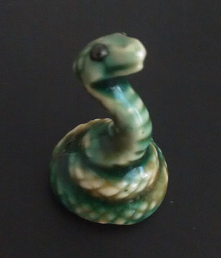
\includegraphics[scale=1]{ular-png}  
	\caption[Gambar {\it Serpentes} dalam format png]{Gambar {\it Serpentes} dalam format png} 
	\label{fig:ularpng} 
\end{figure} 

\dtext{19-20}
\begin{figure}[H]
	\centering  
	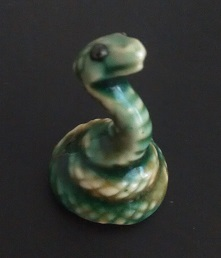
\includegraphics[scale=0.5]{ular-jpg}  
	\caption[Ular kecil]{Ular kecil} 
	\label{fig:ularjpg} 
\end{figure} 
\dtext{21-22}

\begin{figure}[ht] 
	\centering  
	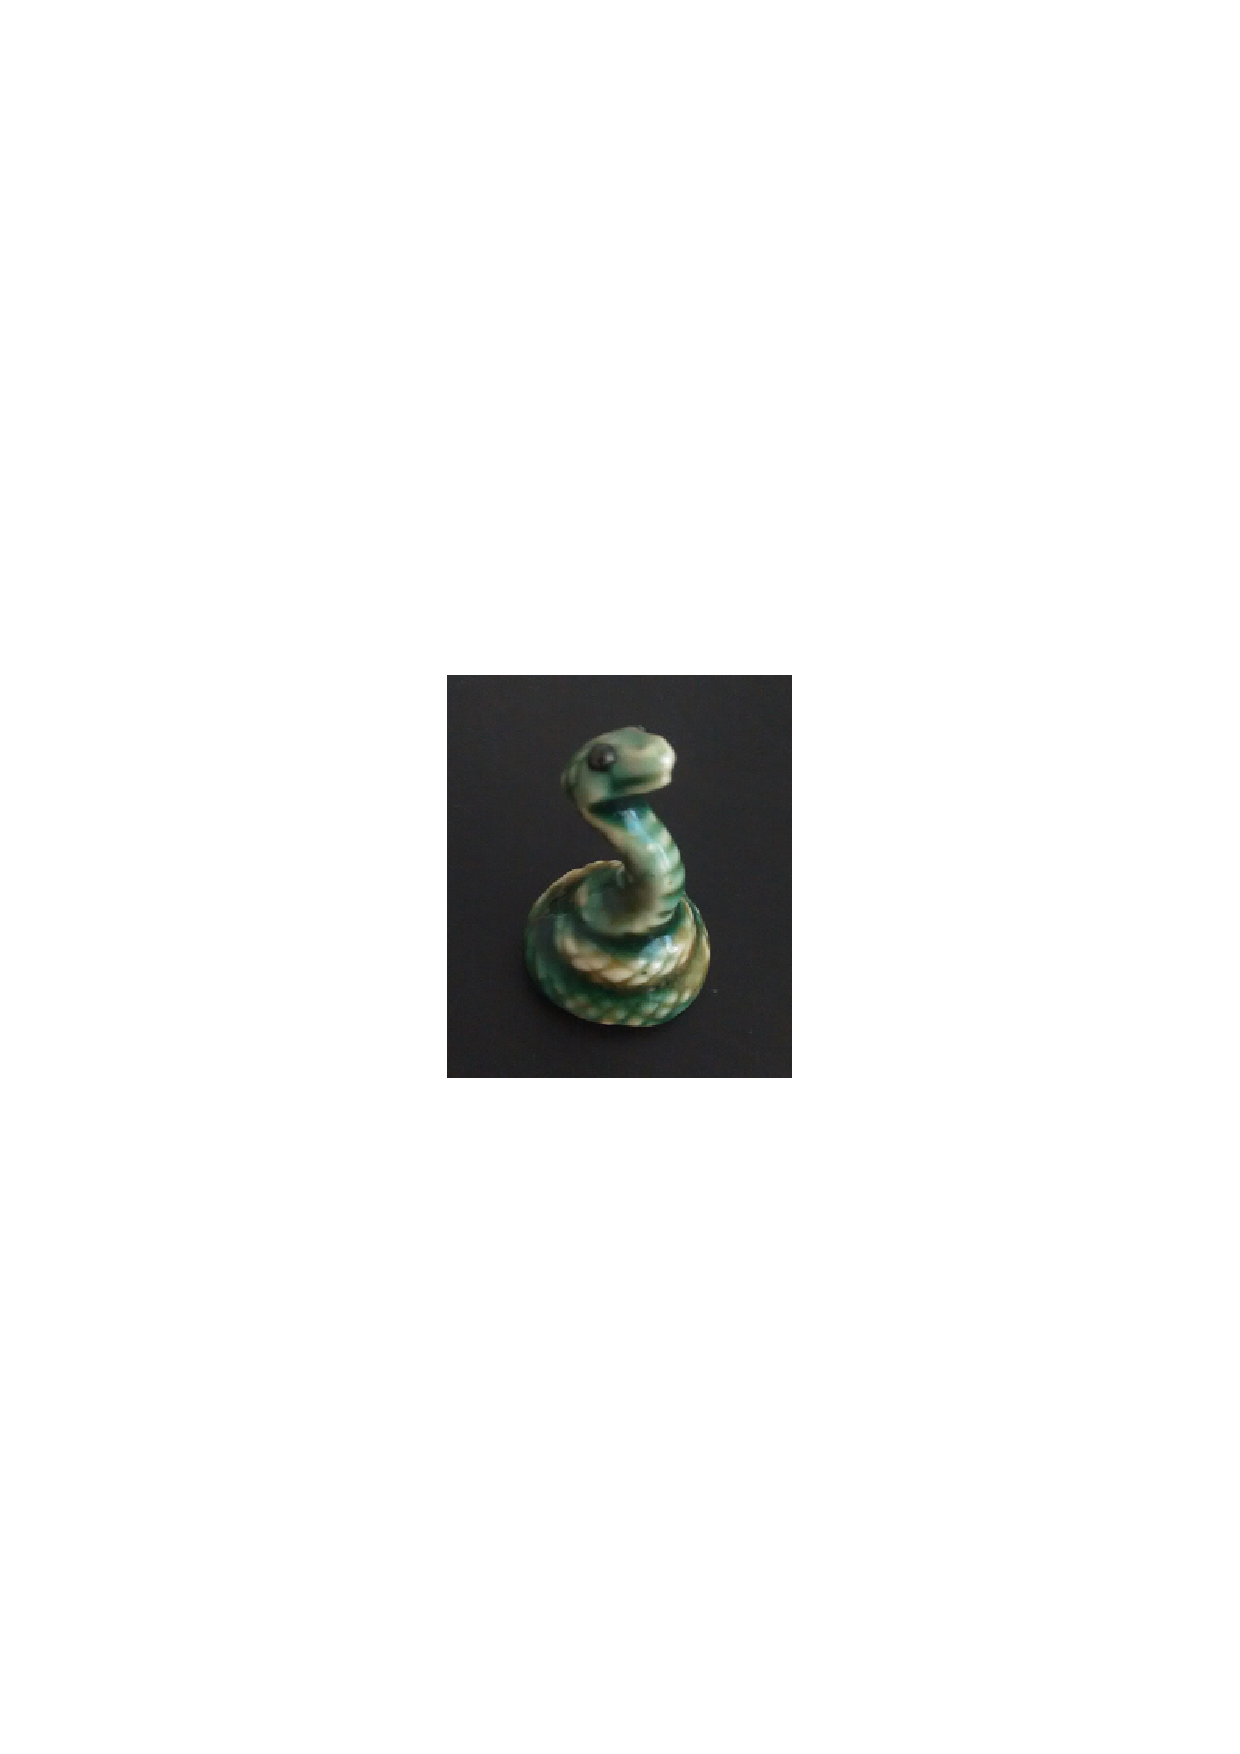
\includegraphics[scale=1]{ular-pdf}  
	\caption[ {\it Serpentes} betina]{ {\it Serpentes} jantan} 
	\label{fig:ularpdf} 
\end{figure} 
 
